\documentclass[border=4pt]{standalone}
\usepackage{tikz}
\usetikzlibrary{arrows.meta,shapes.geometric}
\begin{document}
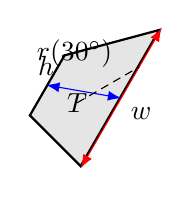
\begin{tikzpicture}[
  >=Latex,
  shape border uses incircle,
  shape border rotate=60,
  every node/.style={text=black}
]
  \node[trapezium,fill=gray!20,draw,thick,minimum width=2cm,
    trapezium left angle=75,trapezium right angle=45] (t) {$T$};
  \draw[red,<->] (t.bottom left corner) -- (t.bottom right corner)
    node[midway,below right] {$w$};
  \draw[blue,<->] (t.top side) -- (t.bottom side)
    node[at start,above] {$h$};
  \draw[densely dashed] (t.center) -- (t.30)
    node[pos=.72,above left] {$r(30^\circ)$};
\end{tikzpicture}
\end{document}
